\documentclass[a4paper,10pt]{article}

\usepackage[brazilian]{babel}
\usepackage[utf8]{inputenc}
\usepackage[T1]{fontenc}
\usepackage{titlesec}
\usepackage{graphicx}
\usepackage{mathtools}
\usepackage{amsthm}
\usepackage[top=1.0in,bottom=1.0in]{geometry}
\usepackage{hyperref}
\usepackage[singlelinecheck=false]{caption}
\usepackage[backend=biber,url=true,doi=true,eprint=false]{biblatex}

\addbibresource{../common/references.bib}

\newcommand\blfootnote[1]{%
  \begingroup
  \renewcommand\thefootnote{}\footnote{#1}%
  \addtocounter{footnote}{-1}%
  \endgroup
}

\titleformat{\section}
  {\normalfont\scshape\bfseries}{\thesection}{1em}{}
\titleformat{\subsection}
  {\normalfont\scshape\bfseries}{\thesubsection}{1em}{}
\titleformat{\paragraph}
  {\normalfont}{\theparagraph}{1em}{}
\titleformat{\subparagraph}
  {\normalfont}{\thesubparagraph}{1em}{}

\captionsetup[table]{labelsep=space}

\theoremstyle{plain}

\newtheorem*{spn-def}{Definição}

\title{\textbf{Modeling and Reasoning with Bayesian Networks: Compiling Bayesian Networks}}

\begin{document}
\date{}
\author{}
\vspace*{-40pt}
{\let\newpage\relax\maketitle}

Relatório semana 1 - MAC0215 (Atividade Curricular em Pesquisa)

Aluno: Renato Lui Geh (Bacharelado em Ciência da Computação)

Orientador: Denis Deratani Mauá

\section{Atividades realizadas na semana}

\paragraph{
  Durante a semana foram lidos os seguintes tópicos do livro \textit{Modeling and Reasoning with
Bayesian Networks}\cite{bayes-net-darwiche}:
}

\begin{description}
  \item[12] - Compiling Bayesian Networks
  \begin{description}
    \item[12.1] - Introduction
    \item[12.2] - Circuit semantics
    \item[12.3] - Circuit propagation
    \begin{description}
      \item[12.3.1] - Evaluation and differentiation passes
    \end{description}
  \end{description}
\end{description}

\section{Definição das atividades}

\paragraph{
  Foram estudados o processo de se compilar Redes Bayesianas em circuitos aritméticos, algumas 
notações usadas em Redes Bayesianas, a definição de uma \textit{network polynomial}, algumas 
propriedades de Redes Bayesianas e diferenciação de uma rede a partir de uma evidência.
}

\paragraph{
  Esta seção será dividida em subseções para cada subtópico citado na seção anterior. Cada 
subseção é um resumo do que foi estudado em cada tópico, contendo os assuntos mais importantes
para o projeto.
}

\subsection{Introduction}

\paragraph{
  Aqui apresentaremos algumas notações usadas em Redes Bayesianas - e que podem ser extendidas para
outros Modelos Gráficos Probabilísticos (PGM).
}

\begin{figure}[h]
\centering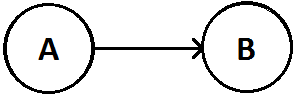
\includegraphics[scale=0.5]{imgs/fig1.png}
\caption{Uma Rede Bayesiana $A \to B$. Em Redes Bayesianas uma aresta representa uma dependência.
  No caso da imagem $A$ depende de $B$. As CPTs associadas a esse grafo estão em Tabela 1 e 
  Tabela 2.}
\end{figure}

\begin{table}[h]
\begin{center}
\captionsetup{justification=centering}
\caption{ e Tabela 2}
\begin{tabular}{c | c}
  A  & $\Theta_A$ \\
\hline
true & $\theta_a = 0.3$ \\
false& $\theta_{\overline{a}} = 0.7$ \\
\end{tabular}
\quad
\quad
\begin{tabular}{c c | c}
A & B & $\Theta_{B|A}$ \\
\hline
true & true & $\theta_{b|a} = 0.1$ \\
true & false & $\theta_{\overline{b}|a} = 0.9$ \\
false & true & $\theta_{b|\overline{a}} = 0.8$ \\
false & false & $\theta_{\overline{b}|\overline{a}} = 0.2$ \\
\end{tabular}
\end{center}
\end{table}

\paragraph{
  Antes de começarmos com circuitos aritméticos, vamos primeiro apresentar algumas definições
importantes.
}

\paragraph{
  Chamamos de CPT (Conditional Probability Table) as tabelas que representam as
probabilidades de uma rede (ex.: as CPTs da Rede Bayesiana na Figura 1 são as Tabelas 1 e 2).
Pode-se claramente ver que para $n$ nós de uma Rede Bayesiana, precisamos de uma quantidade
exponencial $2^n$ de probabilidades para representar cada instância de variáveis.
}

\paragraph{
  Chamamos de MPE (Most Probable Explanation) a instância mais provável de variáveis que aceitam
uma evidência. Mais formalmente dizemos que:
}

\begin{spn-def} Sejam $X_1,...,X_n$ as variáveis da rede e $e$ a evidência dada. Existe uma
  instância $x_1,...,x_n$ onde $Pr(x_1,...,x_n|e)$ é maximal. Chamamos $x_1,...,x_n$ a 
  \textit{explicação mais provável} (\textit{most probable explanation}) dado $e$.
\end{spn-def}

\paragraph{
  Chamamos de MAP (Maximum A Posteriori hypothesis) quando a probabilidade de uma certa instância
é maximal.
}

\begin{spn-def} Sejam $X$ o conjunto de todas as variáveis da rede e $M$ um subconjunto qualquer
  dessas variáveis. Dado uma evidência $e$, qualquer instância $m$ de variáveis $M$ onde $Pr(m|e)$
  é maximal é uma \textit{hipótese máxima a posteriori} (\textit{maximum a posteriori hypothesis}).
\end{spn-def}

\paragraph{
  $M$ também é chamado de variáveis MAP. MPE é uma MAP quando as variáveis MAP incluem todas as
variáveis da rede.
}

\paragraph{
  Agora que temos uma base podemos voltar para circuitos aritméticos. Dado um circuito aritmético 
que representa uma Rede Bayesiana, teremos dois tipos de entradas: variáveis $\theta$, que 
chamaremos de \textit{parâmetros}, e as variáveis $\lambda$, que chamaremos de 
\textit{indicadores}. Parâmetros são valorados de acordo com a CPT da rede, enquanto indicadores
são valorados de acordo com a evidência. Nas próximas subseções veremos que podemos ter duas
passagens pelo circuito. Uma em que vamos de baixo para cima (bottom-up) para calcular a 
probabilidade de uma dada evidência, e outra em que vamos de cima para baixo (top-down), chamada
de \textit{differentiation pass} para calcularmos as derivadas parciais de cada entrada do 
circuito.
}

\subsection{Circuit semantics}


\newpage

\printbibliography

\end{document}
